%%=============================================================================
%% Proof-of-concept: Three.js
%%=============================================================================

\chapter{\IfLanguageName{dutch}{Proof-of-concept: Three.js}{Proof-of-concept: Three.js}}%
\label{ch:proofofconceptThreeJS}

\section{Inleiding}

In dit hoofdstuk zal overlopen worden welke aanpassingen gemaakt zijn aan de conventionele POC. Hierbij zal een kijk genomen worden in hoe deze elementen opgebouwd zijn en welke voordelen ze met zich meebrengen.

Er zijn op twee plaatsen in de webshop aanpassingen gemaakt en dat is op de home pagina en de detail pagina. Voor de implementatie van de componenten is de React Three Fiber bibliotheek gebruikt.

\section{Home pagina}

Voor de home pagina zijn verschillende opties overwogen en uiteindelijk is gekozen voor een interactieve carrousel. Hierbij worden de releases naast elkaar weergegeven zodat de gebruiker intuïtief door de releases kan scrollen.

Onderaan de pagina bevindt zich een minimap die de positie van de gebruiker op de carrousel aangeeft.

De beide componenten bevinden zich in een \texttt{Canvas} die zich over de breedte van de volledige home pagina strekt. Het \texttt{Canvas} is als volgt geïnitialiseerd a.d.h.v. React Three Fiber: 

\newpage

\begin{lstlisting}
<Canvas
	gl={{
			antialias: true,
			toneMapping: THREE.ACESFilmicToneMapping,
			outputEncoding: THREE.sRGBEncoding
	}}
	camera={{ position: [0, 0, 250] }}
	className='canvas'
>
	<HomeScene releases={newReleases?.albums?.items}/>
</Canvas>
\end{lstlisting}

Het \texttt{Canvas} krijgt standaard instellingen mee voor de renderer via de 'gl' property. De camera wordt ook 250 eenheden naar achter geplaatst zodat de objecten in de scene kunnen gezien worden. Binnen in het \texttt{Canvas} wordt een \texttt{HomeScene} component meegegeven met de nodige data voor het tonen van de releases.

\begin{figure}[h]
	\centering
	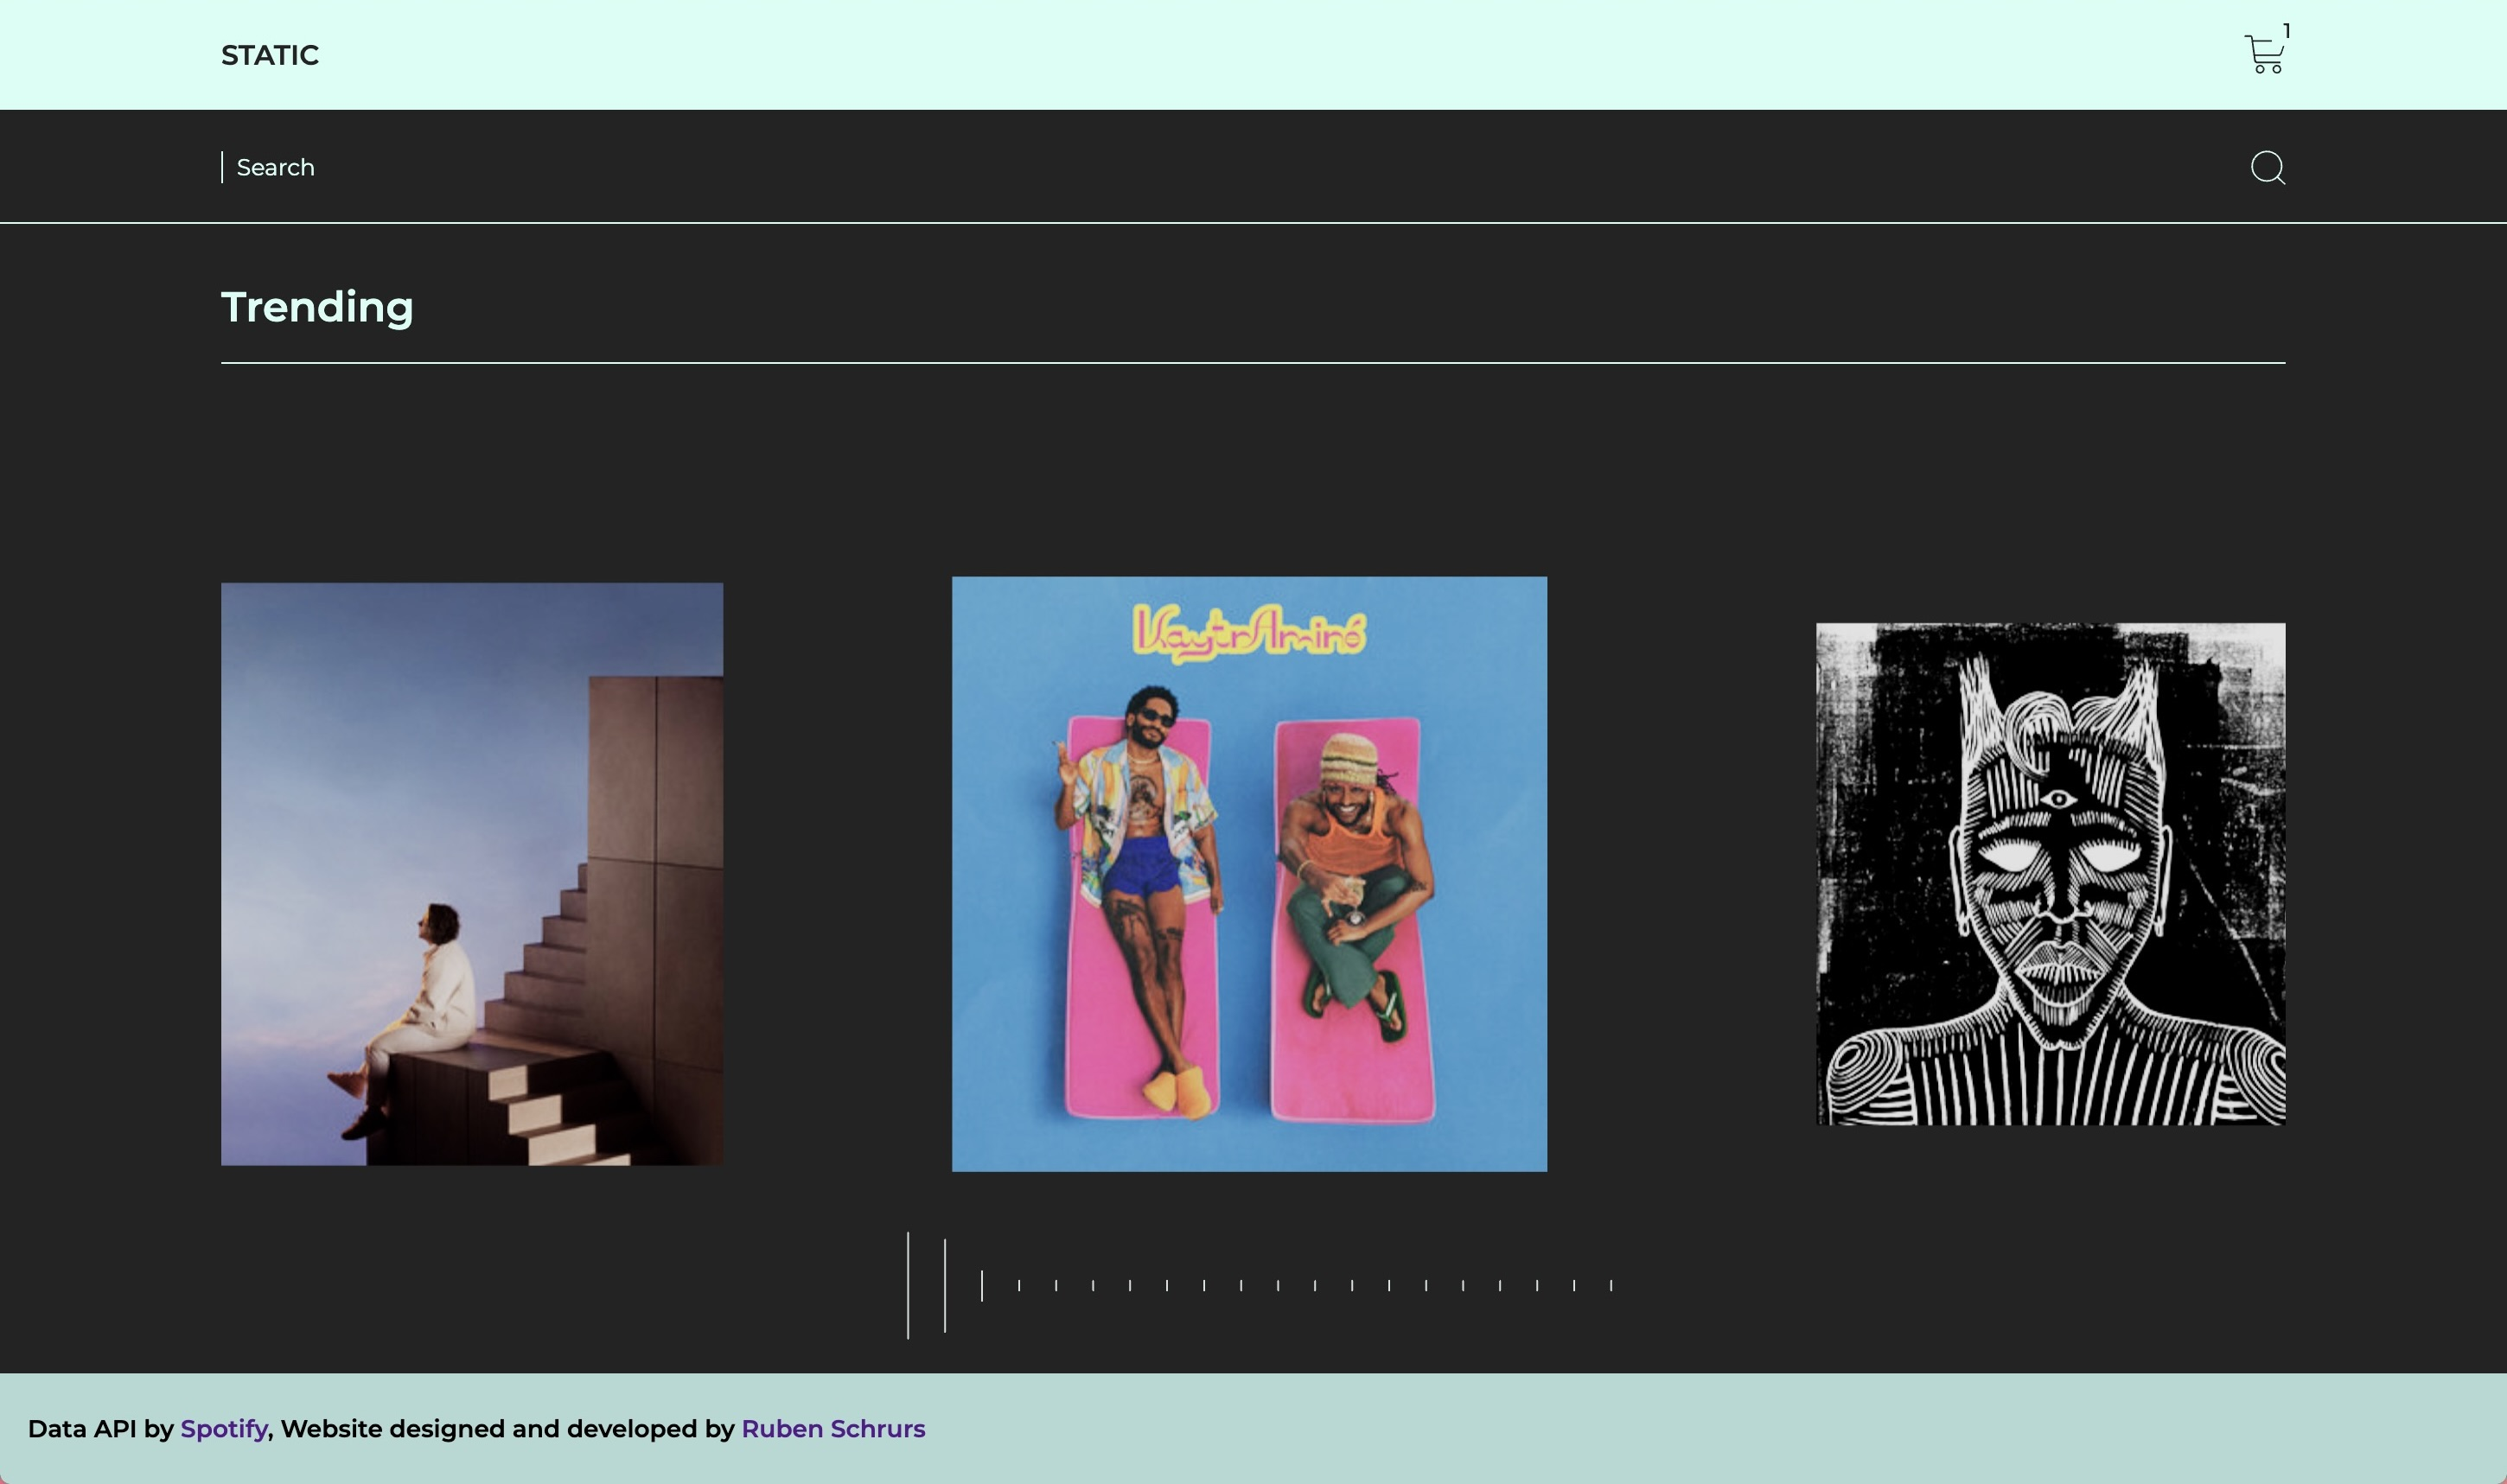
\includegraphics[width=1\linewidth]{graphics/desktopHomeThree}
	\caption[Home pagina Three.js]{Home pagina Three.js}
	\label{fig:desktopHomeThree}
\end{figure}

\newpage
\subsection{HomeScene}

In de \texttt{HomeScene} component worden alle vereiste gegevens doorgegeven om een scene te bouwen. Hieronder vindt u de code voor de renderfunctie van de \texttt{HomeScene}:

\begin{lstlisting}
<directionalLight castShadow position={[0, 0, 1]} />
<ambientLight intensity={0.5} />
<ScrollControls
	pages={(width - xW + totalLength * xW) / width}
	horizontal={!isMobile}
	damping={0.1}
>
	<Scroll>
		<Suspense fallback={<Placeholder position-y={1} scale={[20, 20, 20]} />}>
			<group>
			{
				releases?.map((release, index) => {
					return (
						<ReleaseItem3D
							key={index}
							index={index}
							position={[
								index * xW,
								0, 0
								]}
							scale={scale}
							setScale={setScale}
							release={release}
							totalLength={totalLength}
						/>
					)
				})
			}
			</group>
		</Suspense>
	</Scroll>
	<Minimap items={releases} />
</ScrollControls>
\end{lstlisting}

Als eerste wordt een directioneel licht object meegegeven met de volgende props:

\begin{itemize}
	\item castShadow
	\item position={[0, 0, 1]}
\end{itemize}

De \texttt{castShadow} prop is vanzelfsprekend en zorgt er dus voor dat dit licht object de mogelijkheid krijgt om schaduwen de produceren. De positie van het licht ligt niet in het centrum van de scene omdat de 3D tekst anders moeilijker zichtbaar is. Dit soort licht zal ervoor zorgen dat alle objecten in de scene even belicht zijn vanuit dezelfde richting.

Het volgende licht is een omgevingslicht of \texttt{AmbientLight} object, dit licht zorgt ervoor dat alle vlakken van de 3D tekst zichtbaar zijn. De intensiteit is lager dan de normaal waarde voor een gevoel van perspectief te creëren.

\texttt{ScrollControls} is een van de componenten die beschikbaar wordt gesteld door de bibliotheek react-three/drei. Voor deze component geef je het aantal pagina's door, hiervoor wordt een berekening uitgevoerd op basis van de breedte van de viewport, de lengte van het aantal weergegeven items, en de breedte van elk item plus de opening of 'gap' tussen elk item. De scroll richting kan ook bepaald worden en zal veranderen op basis van de breedte van de viewport. De laatste prop is de 'damping' die bepaald in welke mate de scrollbeweging gedempt wordt.

Alle 3D objecten waardoor gescrolld moet worden worden binnen in een \texttt{Scroll} component geplaatst.

\subsubsection{Carrousel}

In de \texttt{Scroll} component wordt \texttt{Suspense} gebruikt, een native react component, die een fallback zal tonen terwijl de objecten worden ingeladen. In dit geval is dat een \texttt{Placeholder} component die een simpele \texttt{BoxGeometry} is.

Er wordt vervolgens gemapt over de release items en voor elke item een \texttt{ReleaseItem3D} terug gegeven. Hierbij krijgt de component ook de nodige info zoals de positie en schaal.

De \texttt{ReleaseItem3D} component heeft volgende renderfunctie:

\begin{lstlisting}
<group ref={releaseContainer} position={position}>
	<Image 
		ref={releaseImage} 
		scale={scale} url={url} 
		onClick={handleReleaseItem} 
		onPointerOver={over} 
		onPointerOut={out} 
	/>
	{
		hovered ? (
			<group>
				<mesh ref={titleRef} position={[-150, 150, 0]}>
					<textGeometry 
						args={[
							releaseName,
							{ font, size: 15, height: 1 }
						]} 
					/>
					<meshPhysicalMaterial 
						attach='material' 
						color={App.secondaryColor} 
					/>
				</mesh>
				<mesh position={[100, 150, 0]}>
					<textGeometry 
						args={[
							`${price}`,
							{ font, size: 12, height: 1 }
						]} 
					/>
					<meshPhysicalMaterial 
						attach='material' 
						color={App.secondaryColor} 
					/>
				</mesh>
			</group>
		) : (
			null
		)
	}
</group>
\end{lstlisting}

De objecten worden genest in een \texttt{<group>} tag, dit is verplicht bij het gebruik van meerdere R3F componenten en wordt ook gebruikt om de positie van het volledige object te bepalen.
De \texttt{Image} component is een \texttt{react-three/drei} abstractie en krijgt een gepaste schaal mee die afgestemd is op de grootte van de scene alsook de url voor de afbeelding. Wanneer er geklikt wordt op de component dan zal de gebruiker doorverwezen worden naar de detailpagina. Hiernaast wordt ook een boolean bijgehouden of de gebruiker al dan niet hovered over de afbeelding. Indien deze waarde op \texttt{true} komt te staan dan zullen twee 3D text objecten toegevoegd worden in de scene gepositioneerd boven de afbeelding. Linksboven de afbeelding is dat de naam van de release en rechtsboven de prijs, wanneer de naam van de release te lang is dan zal de string waarde afgekapt wordt een beletselteken ingevoegd.

De \texttt{ReleaseItem3D} component bevat een \texttt{useFrame} hook die voor elke frame een nieuwe render zal uitvoeren. 
\newline

\begin{lstlisting}
const scroll = useScroll()

useFrame((state, delta) => {
	const y = scroll.curve(index / totalLength - 1.5 / totalLength, 4 / totalLength)
	
	if (hovered) releaseImage.current.scale.x = damp(
		releaseImage.current.scale.x, 300, 6, delta
	)
	if (hovered) releaseImage.current.scale.y = damp(
		releaseImage.current.scale.y, 300, 6, delta
	)
	
	releaseImage.current.scale[0] = releaseImage.current.scale.x = damp(
		releaseImage.current.scale.x, scale[0] * .6 + scrollValue * 75, 8, delta
	)
	releaseImage.current.scale[1] = releaseImage.current.scale.y = damp(
		releaseImage.current.scale.y, scale[1] * .6 + scrollValue * 75, 8, delta
	)
})
\end{lstlisting}

Op de eerste lijn wordt een \texttt{scrollValue} variabele gedefinieerd die een waarde krijgt op basis van de curve functie van de \texttt{useScroll()} hook. Deze variabele bepaald hoe ver de component ligt t.o.v. het midden waarbij \texttt{scrollValue = 1} als absoluut midden van de scene kan gezien worden. Als de \texttt{hovered} boolean \texttt{true} is dan wordt een animatie uitgevoerd en verandered de schaal van de afbeelding, zie figuur \ref{fig:desktopHomeThreeHovered}. Vervolgens gebruiken we de \texttt{scrollValue} variabele om de schaal van de afbeelding aan te passen wanneer de \texttt{hovered} boolean opnieuw \texttt{false} is, zo keert de schaal terug naar de originele staat. 
Voor beide transformaties wordt gebruik gemaakt van de \texttt{damp()} functie, deze maakt deel uit van het \texttt{MathUtils} object uit de Three.js bibliotheek. De functie zal vloeiend een getal interpoleren van x naar y op een veerachtige manier, dat komt doordat gebruik gemaakt wordt van \texttt{delta} om de beweging onafhankelijk te houden van de beeldsnelheid. De eerste parameter is het startpunt en tweede de doelwaarde, als derde komt de lambda waarde die de snelheid van de veerkracht bepaald waarbij een hogere waarde een snellere transitie zal voortbrengen.

\begin{figure}[h]
	\centering
	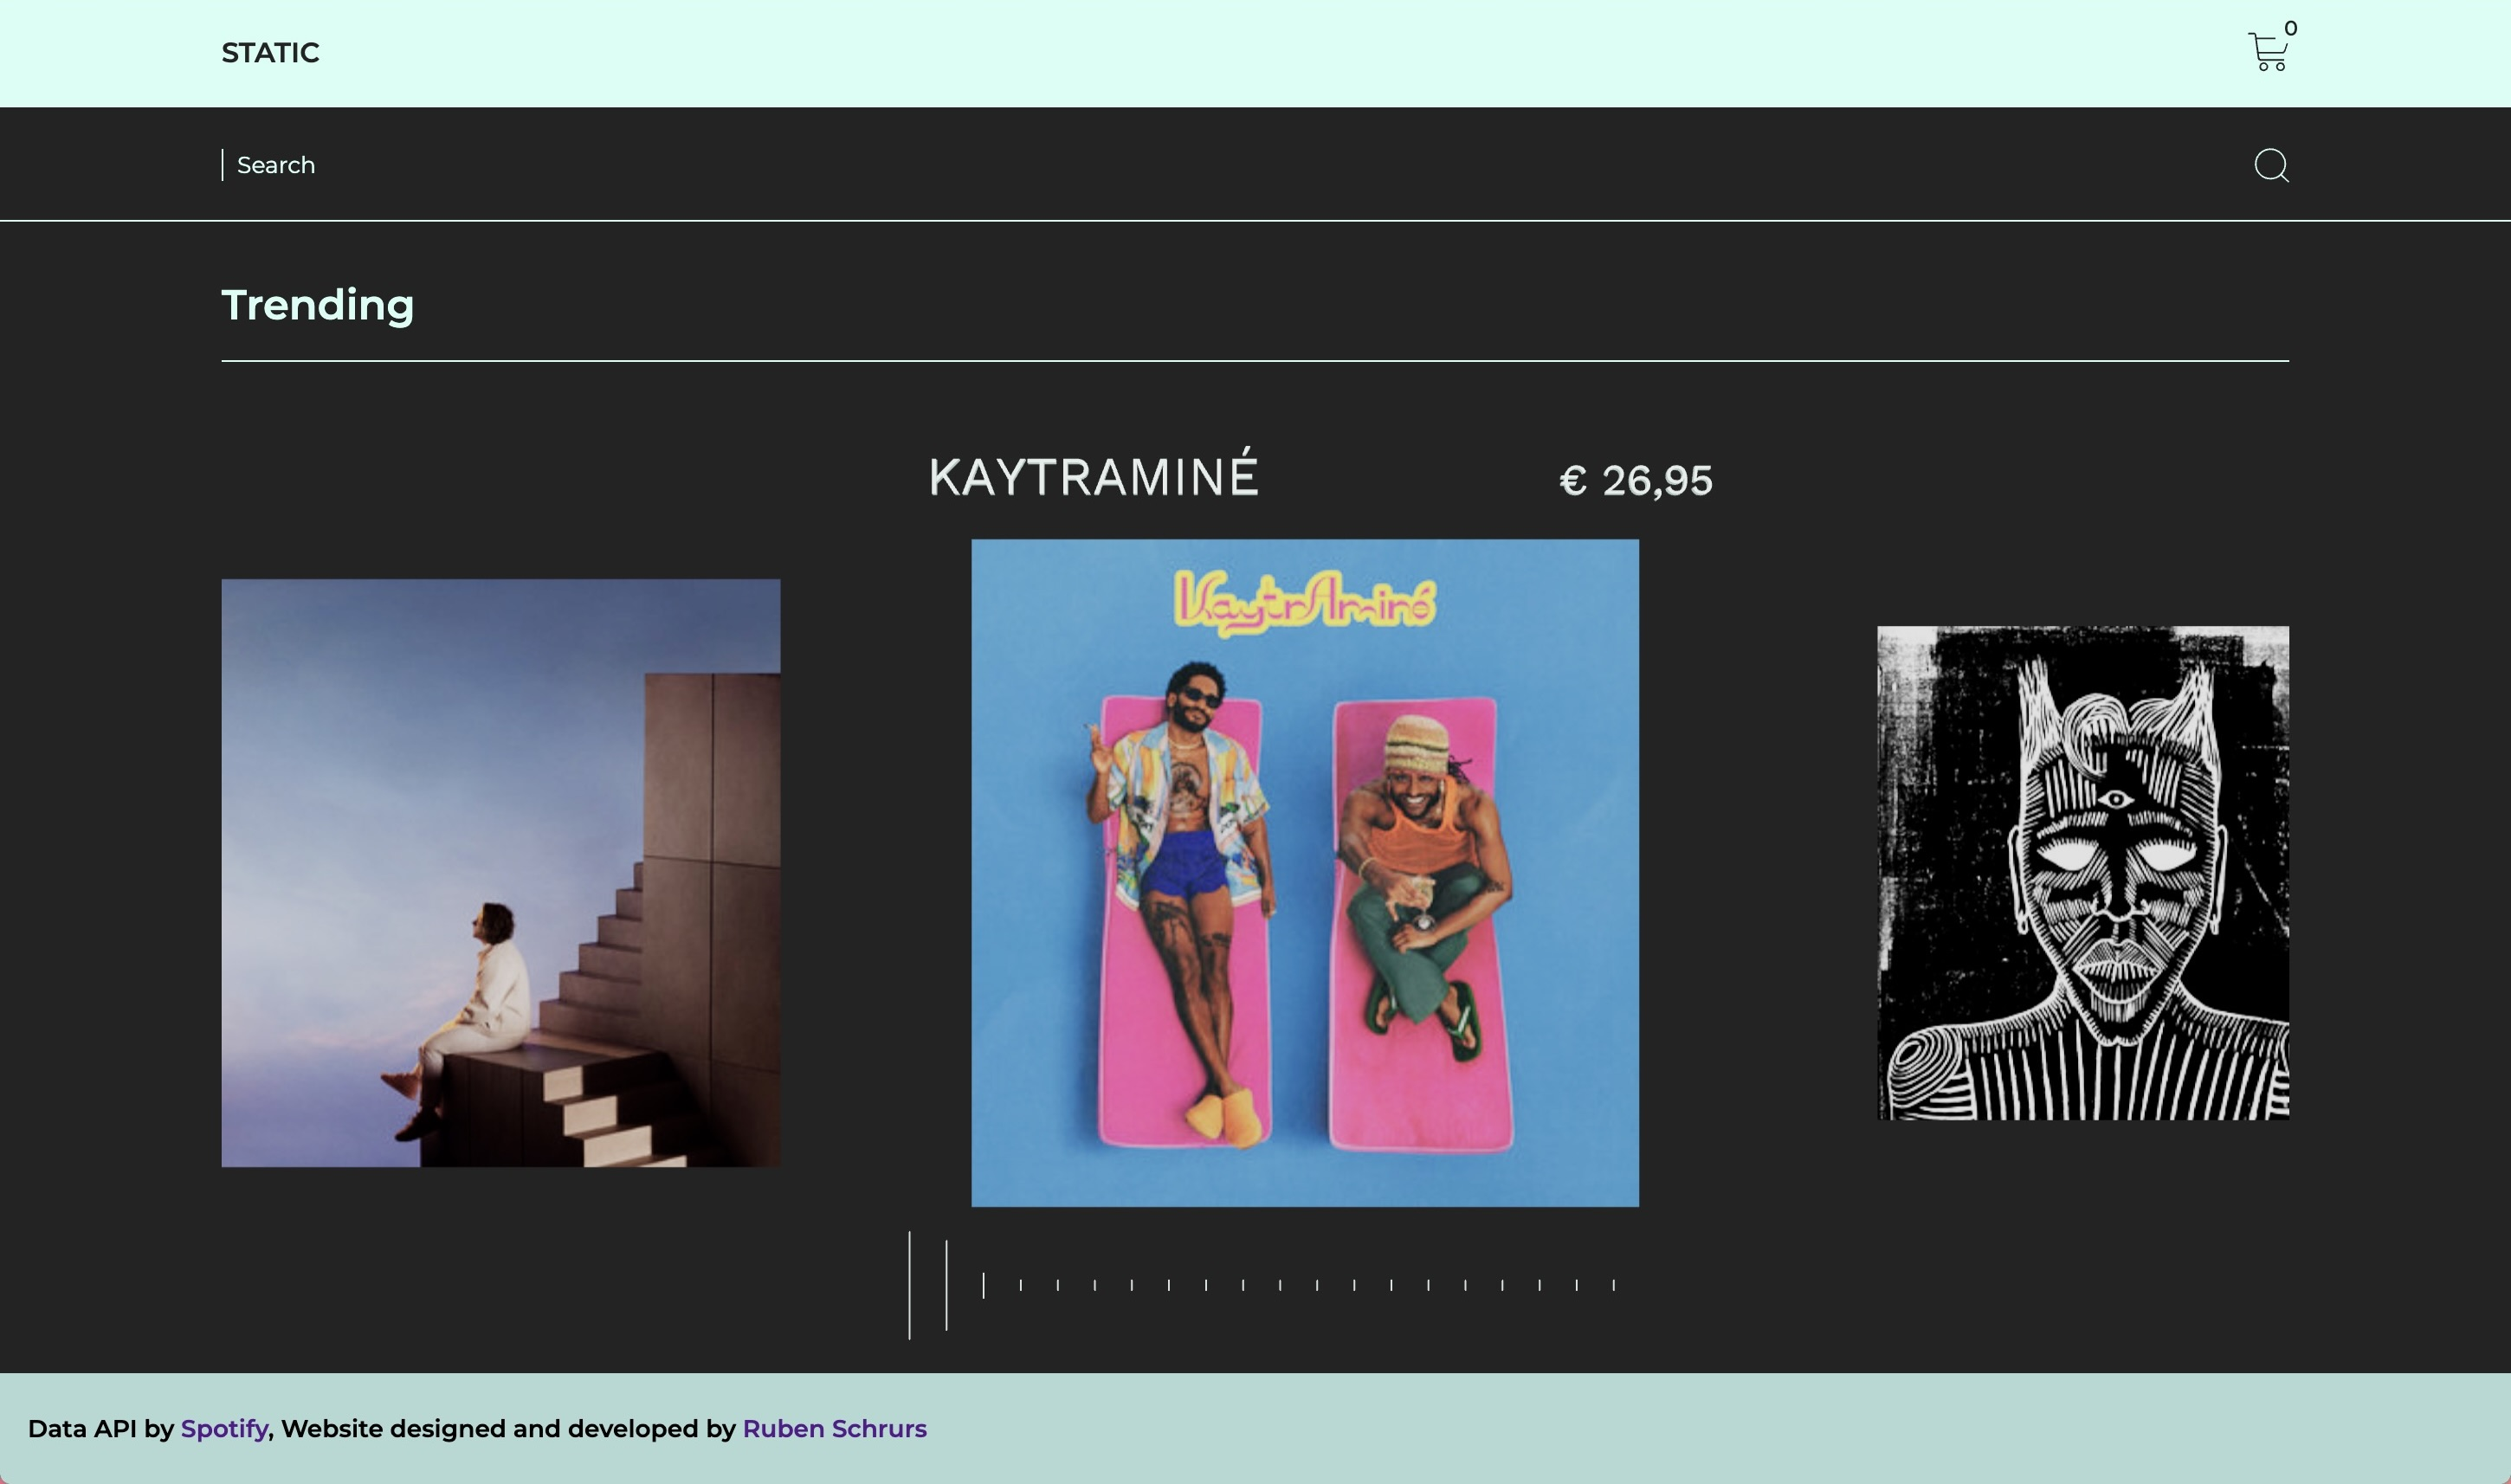
\includegraphics[width=1\linewidth]{graphics/desktopHomeThreeHovered}
	\caption[Home pagina Three.js hovered]{Home pagina Three.js hovered}
	\label{fig:desktopHomeThreeHovered}
\end{figure}
\newpage
\subsubsection{Minimap}

De \texttt{Minimap} component geeft de gebruiker een overzicht over waar die zich bevindt in de carrousel. Dit is gedaan a.d.h.v. verticale lijnen die naast elkaar geplaatst worden. De renderfunctie voor de \texttt{Minimap} component is de volgende: 

\begin{lstlisting}
return (
	<group ref={minimapRef}>
		{items?.map((_, i) => (
			<group 
				key={i} 
				position={[
					i * 15 - items.length * 7,
					- height / 2 + 25,
					-5
				]}
			>
				<Line 
					points={[
						new THREE.Vector3(0, -20, 0),
						new THREE.Vector3(0, 20, 0)
					]} 
					color={App.secondaryColor} 
					lineWidth={1}
				/>
			</group>
			))}
	</group>
)
\end{lstlisting}

Er wordt over de items gemapt die zijn meegegeven aan de \texttt{Minimap} en voor elk item een \texttt{Line} component gegenereerd. De \texttt{Line} bestaat uit twee \texttt{Vector3} objecten en zal tussen deze twee objecten een lijn tekenen met de meegegeven kleur en dikte. Elke lijn krijgt een positie die gebaseerd is op de lengte van het aantal items en de hoogte van de viewport.
Nu alle lijnen gerenderd zijn wordt er ook elke frame een nieuwe render gedaan a.d.h.v. de volgende \texttt{useFrame} hook.

\begin{lstlisting}
useFrame((state, delta) => {
	minimapRef.current.children.forEach((child, index) => {
		const y = scroll.curve(
			index / items.length - 0.15 / items.length,
			4 / items.length
		)s
		child.scale.y = damp(child.scale.y, .1 + y, .8, .2, delta)
	})
})
\end{lstlisting}

In deze useFrame wordt voor elke lijn van de minimap een \texttt{y} variabele gemaakt op basis van het aantal lijnen en de plaats van de individuele lijn. Vervolgens gebruiken we deze om de schaal van de lijn aan te passen met de \texttt{damp()} functie. Deze transformaties zorgen ervoor dat een golf effect over de lijnen wordt geplaatst wanneer de gebruiker scrollt, zie fig. \ref{fig:minimap}.

\begin{figure}[h]
	\centering
	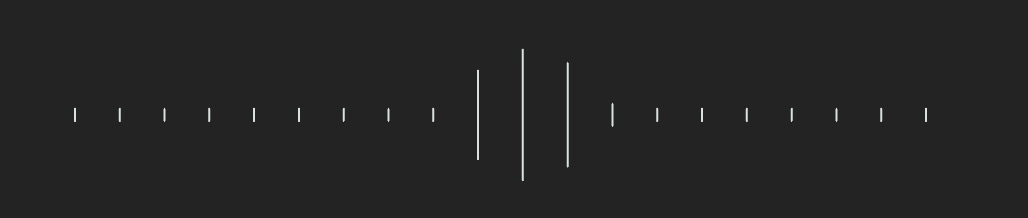
\includegraphics[width=1\linewidth]{graphics/minimap}
	\caption[Minimap]{Minimap}
	\label{fig:minimap}
\end{figure}

\subsection{Hindernissen en uitdagingen}

Het originele idee was om een platenhoes en vinyl plaat in 3D te modelleren en deze dan te importeren in de scene. Dit bleek echter zeer tijdrovend zeker voor een beginner in 3D modelleren. Alhoewel het gelukt is om een platenhoes te modelleren was dat niet het geval voor het plaatsen van een afbeelding op het 3D model. Een van de redenen was omdat het model over meerdere vlakken beschikte, na veel zoeken is dan uiteindelijk gekozen voor een \texttt{PlaneGeometry}. Deze oplossing werd dan opnieuw herzien en vervangen door de \texttt{Image} component uit de \texttt{react-three/drei} bibliotheek.

De 3D tekst is ook een aantal fases ondergaan. Een van de problemen was dat de font die gebruikt wordt over de gehele conventionele versie niet compatibel is. Er vond namelijk af en toe een glitch plaats bij een of meerdere van de letters of cijfers in de font. Niet alle fonts konden dus voor dit project gebruikt worden, na een aantal fonts te proberen is uiteindelijk gekozen voor \texttt{Work Sans Regular}.

\section{Detail pagina}

Het originele idee voor de detail pagina \ref{fig:detailPageThree}was om dezelfde scene te behouden en een animatie te voorzien om tussen de twee pagina's te wisselen. Na een aantal pogingen is toch gekozen voor een de oude scene te verwijderen en een nieuwe in te brengen wanneer een gebruiker op een item klikt.

De hoofdtitel van de detail pagina is dezelfde als de conventionele en bevat ook een link naar de spotify URL voor de release. Verder bevind zich op de linkerhelft van de pagina een 3D representatie van de album cover met een \texttt{ADD TO CART} knop. De rechterhelft van de pagina bevat alle details van de release die ook dezelfde zijn als bij de conventionele versie behalve dat de \texttt{ADD TO CART} knop uiteraard verplaatst is.

\begin{figure}[h]
	\centering
	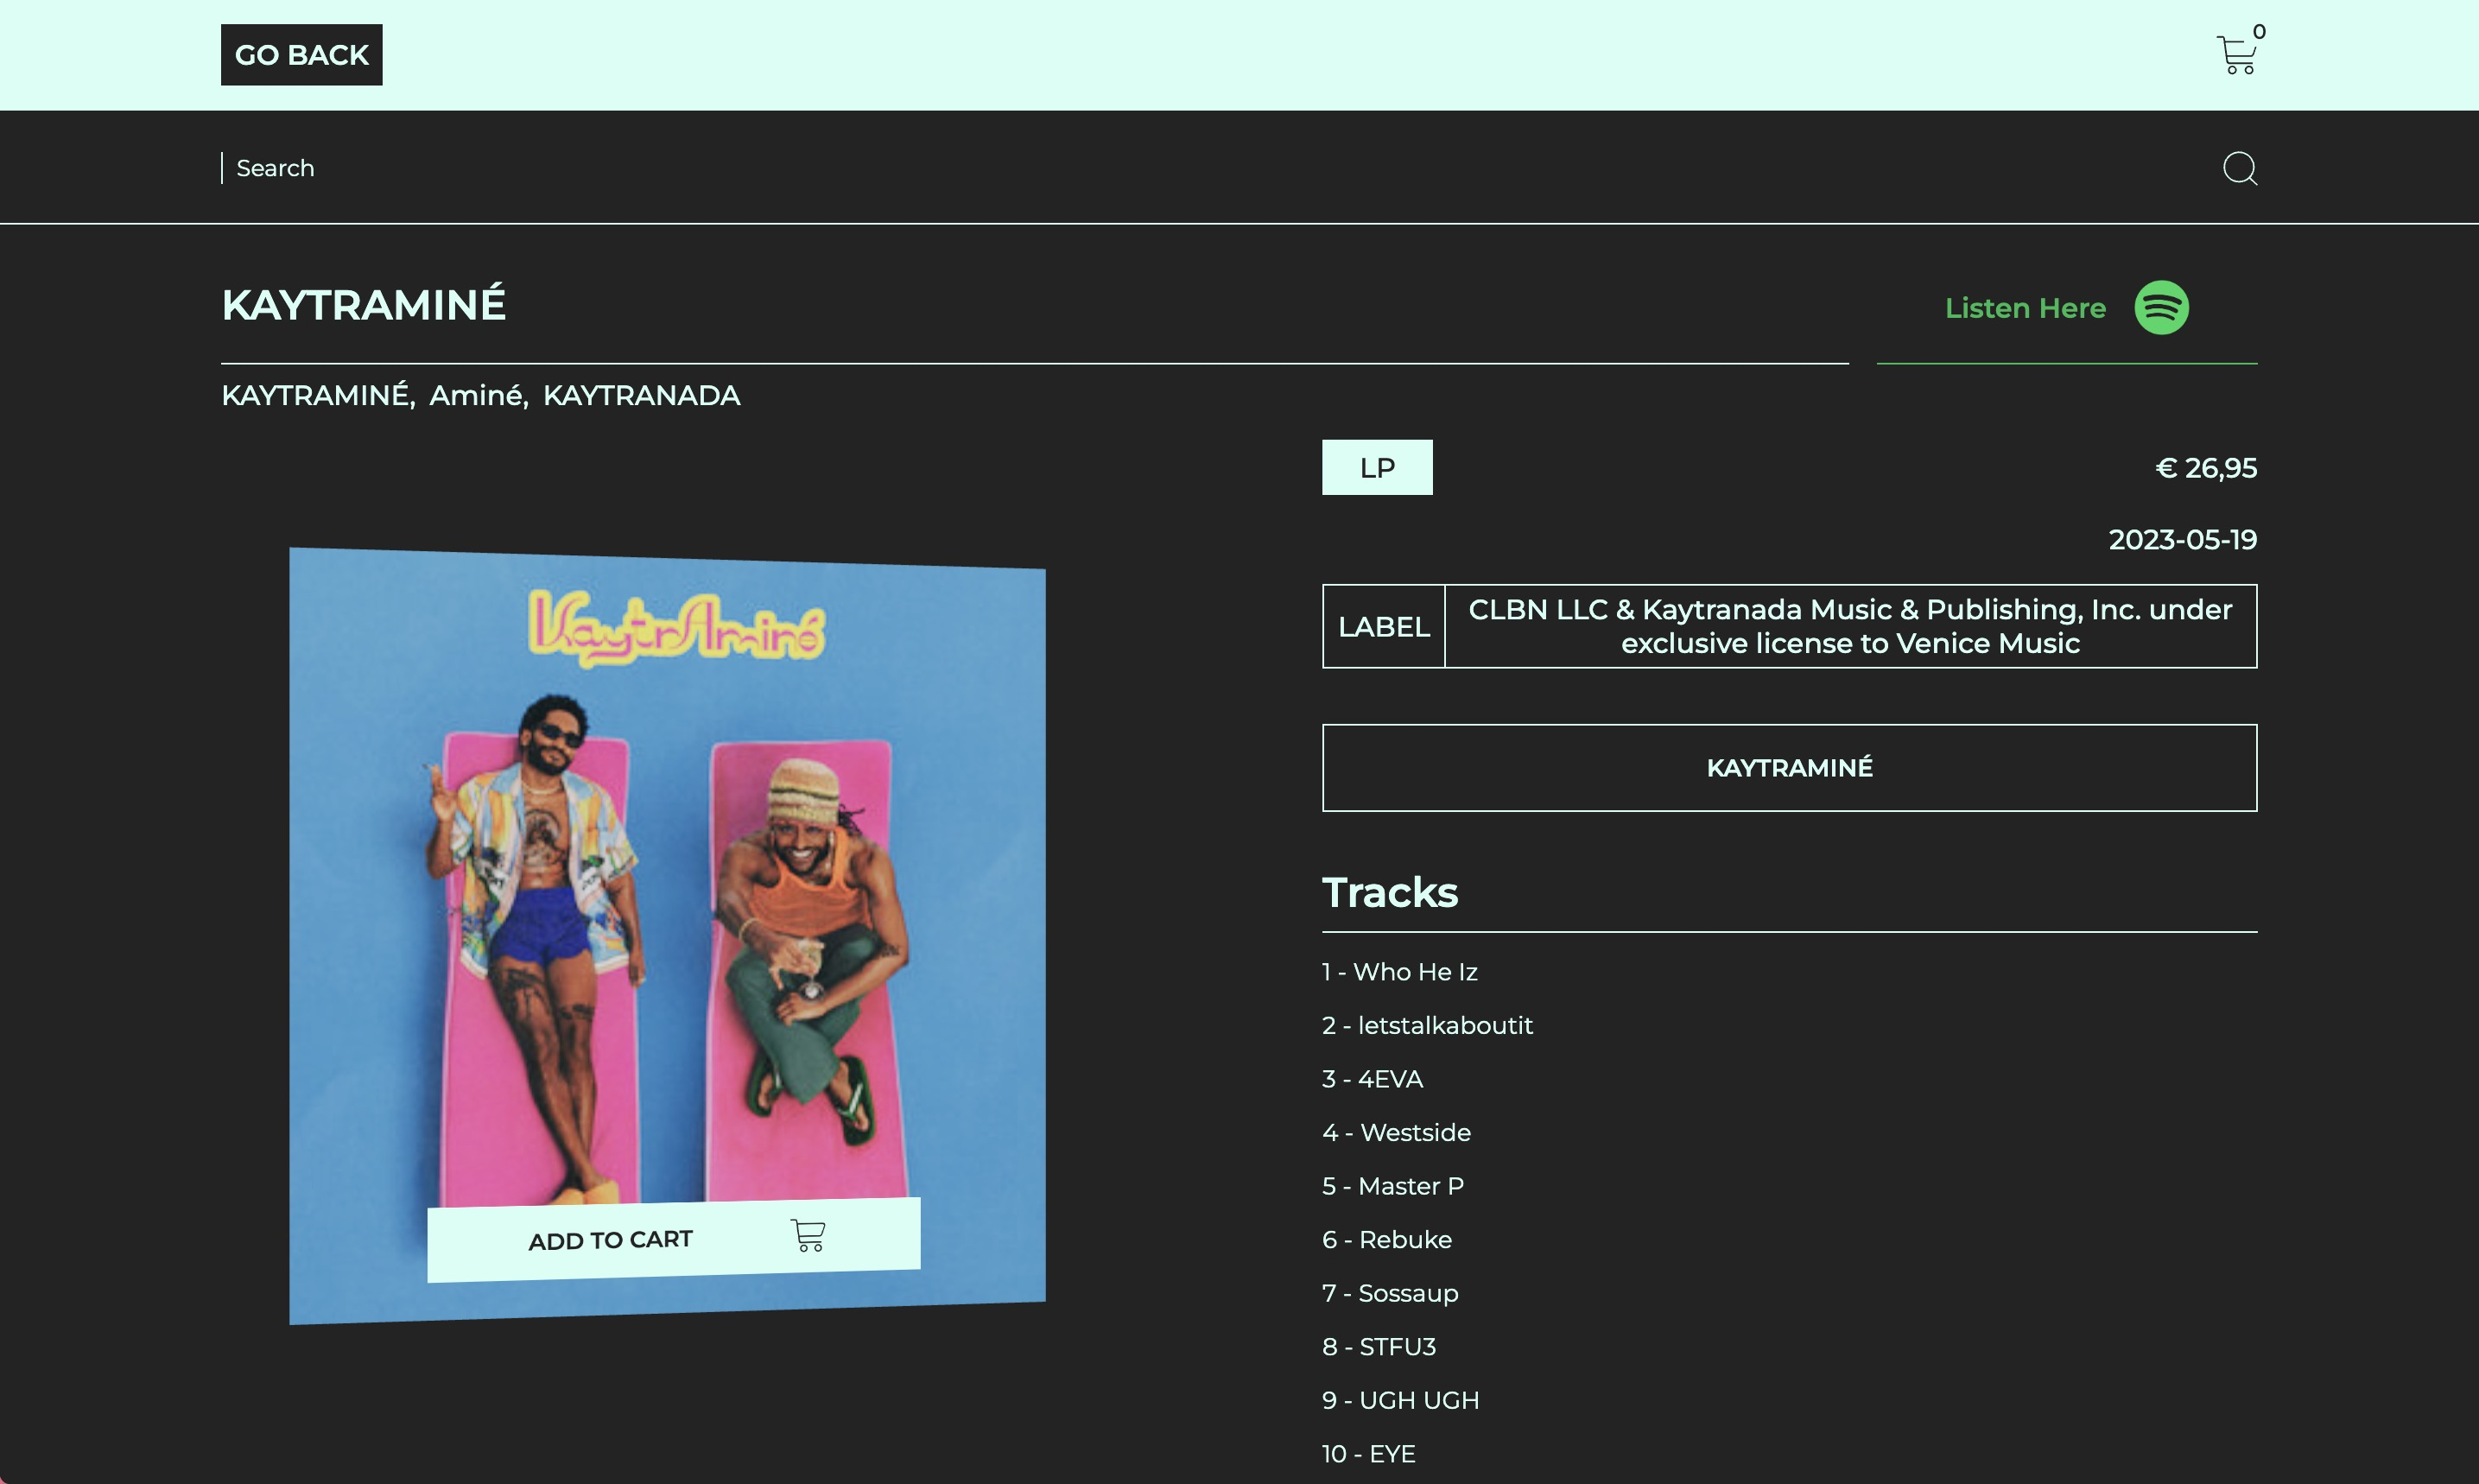
\includegraphics[width=1\linewidth]{graphics/detailPageThree}
	\caption[Detail pagina]{Detail pagina}
	\label{fig:detailPageThree}
\end{figure}

\subsection{DetailsScene}

In deze scene wordt als eerste een directioneel en omgevingslicht ingebracht. Vervolgens zijn ook \texttt{OrbitControls} toegevoegd die in theorie de gebruiker controle geven over de camera. In de \texttt{OrbitControls} component worden echter een aantal props meegegeven om dit af te zetten omdat de gebruiker anders het album object kan verliezen in de scene. Als laatste wordt het \texttt{DetailsItem} geplaatst in een \texttt{Suspense} component voor het inladen van de data.
Deze \texttt{DetailsScene} heeft als doel code te scheiden om een duidelijk overzicht te geven over het inbrengen van licht en besturingstechnieken voor de camera. Alle animaties en transformaties op de 3D modellen worden in de \texttt{DetailItem} component uitgevoerd.

\begin{lstlisting}
return (
	<>
		<directionalLight position={[0, 0, 1]} />
		<ambientLight intensity={0.5} />
		<OrbitControls enableZoom={false} enablePan={false} enableRotate={false}/>
		<Suspense fallback={<Placeholder position-y={1} scale={[20, 20, 20]} />}>
			<group>
				<DetailsItem currentAlbum={currentAlbum} price={price}/>
			</group>
		</Suspense>
	</>
)
\end{lstlisting}

\subsubsection{DetailsItem}

In de \texttt{DetailsItem} is waar de kracht van de \texttt{react-three/drei} bibliotheek uitblinkt. Het nut van deze scene is om de gebruiker een gevoel van controle te geven en zo dus interactief te kunnen omgaan met de website. Dit is gerealiseerd door de volgende functie:
\begin{lstlisting}
function ImageWrapper({ children }) {
	const ref = useRef()
	const vec = new THREE.Vector3()
	const { mouse } = useThree()
	
	useFrame(() => {
		ref.current.position.lerp(vec.set(mouse.x * 15, mouse.y * 15, 0), 0.05)
		ref.current.rotation.y = THREE.MathUtils.lerp(ref.current.rotation.y, (-mouse.x) / 20, 0.1)
	})
	return <group ref={ref}>{children}</group>
}
\end{lstlisting}

De \texttt{ImageWrapper} functie zal de inkomende informatie verwerken en er bewerkingen op uitvoeren. Om te beginnen nemen we de positie van de cursor, hierna wordt de positie van alle kinderen veranderd en voor dit geval is dat alles dat zich in de \texttt{group} tag bevind. De \texttt{lerp()} zal tussen twee waarden lineair interpoleren, de eerste keer dat deze wordt gebruikt is tussen de positie van de kinderen en de positie van de cursor met een factor van 0.05. Voor de rotatie van de kinderen wordt deze een tweede keer gebruikt, nu is dat tussen de huidige rotatie en opnieuw de plaats van de cursor. Op het einde van de functie worden de kinderen teruggegeven en zo wordt de \texttt{ImageWrapper} functie constant opnieuw uitgevoerd. Door deze functie wordt een animatie voorzien die snel kan reageren op de beweging van de gebruiker.

\begin{lstlisting}
return (
	<>
		<group>
			<ImageWrapper>
				<group>
					<mesh>
						<Html
						center
						transform
						scale={18}
						>
							<div className='overlay'>
								<div className='buyButton' onClick={handleBuyButton}>
									<h2>ADD TO CART</h2>
									<svg className="svg-icon" style={svgStyle} viewBox="0 0 1109 1024" version="1.1" xmlns="svgURL" /></svg>
								</div>
							</div>
						</Html>
					</mesh>
					<Image scale={scale} url={currentAlbum?.images[1]?.url} castShadow />
				</group>
			</ImageWrapper>
		</group >
	</>
)
\end{lstlisting}

Binnenin de \texttt{ImageWrapper} zit een \texttt{Html} component en een \texttt{Image} component. Ze komen beiden opniew uit de \texttt{react-three/drei} package, voor het \texttt{Html} gedeelte lijkt het alsof de knop plakt aan de afbeelding en dat is ook het doeleind van deze component. Zo kunnen html elementen die normaal niet in een scene geplaatst kunnen worden toch geïmplementeerd worden. De knop werkt exact hetzelfde als de knop in de conventionele versie van de POC, voor de afbeelding is ook dezelfde methode gebruikt als in de home pagina.

\subsection{Hindernissen en uitdagingen}

Zoals eerder al vermeld is was het de bedoeling om een volledig aaneenhangende ervaring te creëren tussen de home pagina en detail pagina maar dit bleek net een stap te veel te zijn. Om dit te doen moet namelijk van niet alleen van camera maar ook van controls gewisseld worden. Er zijn een aantal versies geweest van de detailpagina waar ook de prijs en LP box zich in de overlay bevonden. Dit bleek echter een moeilijk gegeven, wanneer er een aanpassing was aan de viewport dan was de overlay niet meer correct.

